%%%%%%%%%%%%%%%%%%%%%%%%%%%%%%%%%%%%%%%%%%%%%%%%%%%%%%%%%%%%%%%%%%%%%%%%%%%%%%%%%%
%%%%%%%%%%%%%%%%%%%%%%%%%%%%%%%%%%%%%%%%%%%%%%%%%%%%%%%%%%%%%%%%%%%%%%%%%%%%%%%%%%
\section{Introduction}
%%%%%%%%%%%%%%%%%%%%%%%%%%%%%%%%%%%%%%%%%%%%%%%%%%%%%%%%%%%%%%%%%%%%%%%%%%%%%%%%%%
%%%%%%%%%%%%%%%%%%%%%%%%%%%%%%%%%%%%%%%%%%%%%%%%%%%%%%%%%%%%%%%%%%%%%%%%%%%%%%%%%%

In this paper, we present a Diffusion Synthetic Acceleration (DSA) scheme
that is fully compatible with the Piece-Wise Linear Discontinuous (PWLD) finite
element discretization of the transport equation on arbitrary
polygonal cells. 

Arbitrary polygonal (polyhedral in 3D) cells can advantageously be employed, especially
in the context of spatial discretizations based on discontinuous finite elements (DFE),
for the following reasons: polygonal grids 
\ben
\item may allow for a reduced numbers of unknowns and
\item can provide a natural transition for locally adapted meshes. 
\een
To illustrate these two points, first consider
a hexagonal cell. Employing a PWLD discretization, such a cell possesses six unknowns. Using
alternate discintinuous finite element discretizations that perform well in the thick diffusive limit, such as 
linear discontinuous on triangles and bilinear discontinuous on quadrangles, the same 
hexagonal cell could be split into two quadrangles (for a total of 8 unknowns), two 
triangles and one quadrangle (10 unknowns), or four triangles (12 unknowns). By inserting an 
extra point inside the cell, the hexagon could also be divided into three quadrangles 
(12 unknowns), four quadrangles (16 unknowns) or six triangles (18 unknowns). A 
similar reasoning can be applied to any $n$-polygon. Arbitrary polygonal grids can 
also handle locally refined meshes in a natural manner. The example given
in \Cref{fig_amr} is typical of configurations obtained with Adaptive Mesh 
Refinement (AMR), where neighboring cells possess different refinement level depths. 
Solvers based on arbitrary polygonal cells can easily handle cells 
with various numbers of edges as follows: on \Cref{fig_amr}, the left cell is actually interpreted 
as a (degenerate) pentagon whereas the two cells on the right are quadrilaterals. The PWLD spatial
discretization can handle locally adapted meshes without any special treatment 
or further approximation of the coupling between cells. Moreover, the finite element representation
on the refined side is piece-wise linear. Had the finite element representation been, for instance,
bilinear discontinuous (BLD), the unrefined cell in \Cref{fig_amr} would remain rectangular with a linear
(not piece-wise linear) representation of the solution along the refined edge. 
\begin{figure}[H]
   \centering
   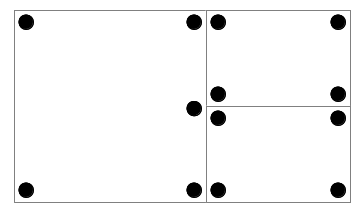
\includegraphics[width=0.3\textwidth]{fig_amr.png}
   \caption{Adaptive mesh refinement grid with PWLD finite elements: left cell is interpreted as a pentagon while right cells are quadrangles.}
   \label{fig_amr}
\end{figure}


%%%%%%%%%%%%%%%%%%%%%%%%%%%%%%%%%%%%%%%%%%%%%%%%%%%%%%%%%%%%%%%%%%%%%%%%%%%%%%%%%%
%\subsection{Rationale for DSA preconditioning}
%%%%%%%%%%%%%%%%%%%%%%%%%%%%%%%%%%%%%%%%%%%%%%%%%%%%%%%%%%%%%%%%%%%%%%%%%%%%%%%%%%

Next, we recall the rationale for solving transport problems iteratively using 
diffusion acceleration schemes (preconditioners).
Because analytical solutions are unavailable for most
radiation transport problems of practical interest, one typically employs
iterative techniques to solve the large system of equations that results from
the spatial and angular discretizations of the transport equation. Standard
iterative techniques for the first-order form of the discrete-ordinate (\sn)
transport equation include Source Iteration (SI)  and Krylov 
subspace techniques (usually GMRes \cite{gmres}). For highly diffusive materials 
(i.e., with scattering ratios $c=\Sigma_s / \Sigma_t $ close to 1) and optically 
thick configurations (i.e., problems that are not leakage-dominated), these iterative techniques 
can become quite ineffective, requiring high iteration counts and possibly 
leading to false convergence. To mitigate these issues, SI and GMRes-based transport solves 
can be effectively accelerated (preconditioned) using Diffusion Synthetic Acceleration (DSA) 
\cite{dsa_ref,larsen_dsa,consistent_p1,m4s,wla,mip}. 

The spatial discretization of the DSA equations
must be somewhat ``consistent'' with the one used for the \sn transport equations 
in order to yield unconditionally stable and efficient DSA schemes
\cite{dsa_ref,larsen_dsa,consistent_p1,m4s,wla,mip}. However, the search for full
consistency between the discretized transport equations and the discretized
diffusion may not be computationally practical (especially for unstructured
arbitrary meshes, \cite{dsa_ref}). For instance, Warsa, Wareing, and
Morel \cite{consistent_p1} derived a fully consistent DSA scheme for linear
discontinuous finite elements on unstructured tetrahedral meshes; their DSA
scheme yields a $P_1$ system of equations that is
computationally more expensive than partially consistent DSA schemes that are
based upon discretizations of a standard diffusion equation. Several partially 
consistent schemes have been analyzed for discontinuous finite element
discretizations of the transport equation on unstructured meshes, for
example, the modified-four-step (M4S) scheme \cite{m4s}, the
Wareing-Larsen-Adams (WLA) scheme \cite{wla}, and the Modified Interior
Penalty (MIP) scheme \cite{mip}.

%%%%%%%%%%%%%%%%%%%%%%%%%%%%%%%%%%%%%%%%%%%%%%%%%%%%%%%%%%%%%%%%%%%%%%%%%%%%%%%%%%
%\subsection{PWLD discretization on arbitrary grids}
%%%%%%%%%%%%%%%%%%%%%%%%%%%%%%%%%%%%%%%%%%%%%%%%%%%%%%%%%%%%%%%%%%%%%%%%%%%%%%%%%%

%% Several discretization methods haven been developed for 
%% arbitrary polygonal meshes \cite{pwld_2d,pwld_3d,cfm_dfm,pwl_diffusion,
%% palmer_fe,mimetic,cell_centered_diff,palmer_proc,palmer_ane,wachspress,pwbld}.
%% In this work, we focus on the PWLD discretization because it was successfully
%% used to discretize the transport equation \cite{pwld_2d,pwld_3d}. This
%% discretization can be applied for any polygonal cells and the integrals
%% generated by this discretization can be easily computed analytically. 

To the authors' knowledge, no work is currently ongoing to adapt the M4S 
technique to polygonal meshes. This is very likely due to the fact
that the M4S scheme does not yield a Symmetric Positive Definite (SPD)
matrix and was found to be divergent for 3D tetrahedral meshes with linear 
discontinuous elements \cite{consistent_p1}. 
% 
Recent work to develop a DSA scheme for polygonal cells has mainly focused 
on adapting the WLA scheme to polygonal meshes
\cite{cfm_dfm,wla_pwl}. The WLA scheme is a two-stage process, where first a
diffusion solution is obtained using a {\em continuous} finite element
discretization and then a {\em discontinuous} update is performed cell-by-cell 
in order to provide an appropriate discontinuous scalar flux correction to 
the discontinuous finite element transport 
solver. In \cite{consistent_p1}, the WLA scheme was
found to be a stable and effective DSA technique, though its efficiency
degraded as the problem became optically thick and highly diffusive.
%
In this paper, we extend the MIP technique to the
PWLD discretization technique for arbitrary polygonal meshes.
The MIP scheme is based on the standard Interior Penalty (IP) method for the
discontinuous finite element discretization of diffusion equations. MIP was first derived in
\cite{mip}, where it was applied to triangular unstructured meshes (with
locally adapted cells). MIP does not suffer from the same issues as the WLA technique when the
problem becomes optically thick and highly diffusive and, therefore, can be a
useful alternate DSA for to accelerate DFE transport solves. 
%Because MIP produces an SPD matrix, the authors of \cite{mip}
%have solved the resulting linear system using a Preconditioned Conjugate Gradient (PCG) technique
In \cite{mip}, a Preconditioned Conjugate Gradient (PCG) technique (with Symmetric Gauss-Seidel, 
SGS, as preconditioner) was used to solve the MIP-DSA equation. In this paper, we also analyze  
the effectiveness of algebraic multigrid methods (AMG) \cite{amg,amg_course} as a preconditioner. 
%the MIP-DSA diffusion solve and we compare AMG with PCG. %+\textcolor{red}{SGS/SSOR}.
%Algebraic multigrid methods allow the use of multigrid techniques when no grid
%information is available or when the grid is unstructured. Instead of using a
%succession of grids based on the geometry of the problems, the ``grid levels''
%are based on properties of the matrix.

The remainder of this paper is organized as follows. In \Cref{sec_transport},
we briefly review the PWLD discontinuous finite element discretization 
and the iterative solution techniques applied to the 
\sn transport equation. 
The MIP-DSA scheme is extended to the PWLD discretization for arbitrary 
polygons in \Cref{sec_mip}. In \Cref{sec_amg}, we introduce the Algebraic MultiGrid (AMG) 
approaches used here, which are based on the ML package of Trilinos \cite{ml_guide} and the
AGMG (AGgregation-based algebraic MultiGrid) technique of 
\cite{agmg_guide,agmg,agmg2,agmg3}. In
\Cref{sec_res}, we present a Fourier analysis for the MIP-DSA scheme discretized with
PWLD, and we compare the different preconditioned CG approaches.
Conclusions are given in \Cref{sec_conc}.
